              %******************************************%
              %                                          %
              % Modello di tesi di laurea o di dottorato %
              %            di Lorenzo Pantieri ©         %
              %                                          %
              %        versione: 23 dicembre 2011        %
              %                                          %
              %******************************************%


% I seguenti commenti speciali impostano:
% 1. utf8 come codifica di input,
% 2. PDFLaTeX come motore di composizione;
% 3. Tesi.tex come documento principale;
% 4. il controllo ortografico italiano per l'editor.

\documentclass[10pt,%                      % corpo del font principale
               a4paper,%                   % carta A4
               twoside,openright,%         % fronte-retro
               titlepage,%                 % frontespizio
               headinclude,,footinclude,%  % testatina e piè di pagina
               BCOR5mm,%                   % rilegatura di 5 mm
               cleardoublepage=empty,%     % pagine vuote senza testatina e piè di pagina
               tablecaptionabove,%         % didascalie in cima alle tabelle
               dottedtoc%                  % puntini nell'indice
               ]{scrreprt}                 % classe report di KOMA-Script;

%\documentclass[10pt,%                      % corpo del font principale
%               a4paper,%                   % carta A4
%               twoside,openright,%         % fronte-retro
%               ]{book}

\usepackage[T1]{fontenc}                   % codifica dei font

\usepackage[utf8]{inputenc}                % codifica di input

\usepackage{microtype}                     % microtipografia

\usepackage[italian,english]{babel}        % per scrivere in italiano e in inglese;
                                           % l'ultima lingua (l'italiano) è predefinita

\usepackage[binding=5mm]{layaureo}         % margini ottimizzati per l'A4; rilegatura di 5 mm

\usepackage[suftesi]{frontespizio}         % frontespizo

\usepackage{emptypage}                     % pagine vuote senza testatina e piè di pagina

\usepackage{indentfirst}                   % rientra il primo paragrafo di ogni sezione

\usepackage{booktabs}                      % tabelle

\usepackage{tabularx}                      % tabelle di larghezza prefissata

\usepackage{graphicx}                      % immagini

\usepackage{subfig}                        % sottofigure, sottotabelle

\usepackage{caption}                       % didascalie

\usepackage{listings}                      % codici

\usepackage[font=itshape,font+=small]{quoting}           % citazioni

\usepackage{amsmath,amssymb,amsthm}        % matematica

\usepackage{varioref}             % riferimenti completi della pagina

\usepackage{mparhack,fixltx2e,relsize}     % finezze tipografiche

\usepackage[style=philosophy-modern,hyperref,backref,square,natbib]{biblatex}
                                           % eccellente pacchetto per la bibliografia;
                                           % lo stile di citazione è autore-anno;
                                           % lo stile "numeric-comp" dà riferimenti numerici

\bibliography{Bibliografia}                % database di biblatex

\usepackage{chngpage,calc}                 % centra il frontespizio
 
\usepackage[dvipsnames]{xcolor}            % colori

\usepackage{lipsum}                        % testo fittizio

\usepackage{eurosym}                       % simbolo dell'euro

\usepackage[printonlyused]{acronym}        % acronimi

\usepackage{hyperref}                      % collegamenti ipertestuali


\usepackage[eulerchapternumbers,%          % numeri dei capitoli nel font Euler
            subfig,%                       % compatibilitˆ con subfig
            beramono,%                     % Bera Mono come font a spaziatura fissa
            eulermath,%                    % AMS Euler come font per la matematica
            pdfspacing,%                   % migliora il riempimento di riga
            listings,%                     % codici
%           parts,%                        % da decommentare se il documento è diviso in parti
            ]{classicthesis}               % stile ClassicThesis

\usepackage{arsclassica}                   % modifica alcuni aspetti di ClassicThesis




\usepackage{bookmark}                      % segnalibri

\usepackage[lined,boxed]{algorithm2e}
\usepackage{multicol}


%*********************************************************************************
% impostazioni-tesi.tex
% di Lorenzo Pantieri (2011)
% file che contiene le impostazioni della tesi
%*********************************************************************************


%*********************************************************************************
% Comandi persaonali
%*******************************************************
\newcommand{\myName}{Riccardo Volonterio}                       % autore
\newcommand{\myTitle}{Web-based Human- and Machine-Driven computation} % titolo
\newcommand{\myDegree}{Tesi di laurea specialistica}                       % tipo di tesi
\newcommand{\myUni}{Politecnico di Milano} % università
\newcommand{\mySede}{Polo regionale di Como}    % facoltà
\newcommand{\myFaculty}{Facoltà di Lettere e Filosofia}    % facoltà
\newcommand{\myDepartment}{Dipartimento di Elettronica e Informazione}         % dipartimento
\newcommand{\myProf}{Alessandro Bozzon}      % relatore
\newcommand{\myOtherProf}{Luca Galli}              % correlatore (se c'è)
\newcommand{\myLocation}{Como}                         % dove
\newcommand{\myTime}{Settembre 2012}                          % quando



%*********************************************************************************
% Impostazioni di amsmath, amssymb, amsthm
%*********************************************************************************

% comandi per gli insiemi numerici (serve il pacchetto amssymb)
\newcommand{\numberset}{\mathbb}
\newcommand{\N}{\numberset{N}}
\newcommand{\R}{\numberset{R}}

% un ambiente per i sistemi
\newenvironment{sistema}%
  {\left\lbrace\begin{array}{@{}l@{}}}%
  {\end{array}\right.}

% definizioni (serve il pacchetto amsthm)
\theoremstyle{definition}
\newtheorem{definizione}{Definizione}

% teoremi, leggi e decreti (serve il pacchetto amsthm)
\theoremstyle{plain}
\newtheorem{teorema}{Teorema}
\newtheorem{legge}{Legge}
\newtheorem{decreto}[legge]{Decreto}
\newtheorem{murphy}{Murphy}[section]



%*********************************************************************************
% Impostazioni di biblatex
%*********************************************************************************
\defbibheading{bibliography}{%
\cleardoublepage
\phantomsection
\addcontentsline{toc}{chapter}{\bibname}
\chapter*{\bibname\markboth{\bibname}
{\bibname}}}



%*********************************************************************************
% Impostazioni di listings
%*********************************************************************************
\lstset{language=[LaTeX]Tex,%C++,
    keywordstyle=\color{RoyalBlue},%\bfseries,
    basicstyle=\small\ttfamily,
    %identifierstyle=\color{NavyBlue},
    commentstyle=\color{Green}\ttfamily,
    stringstyle=\rmfamily,
    numbers=none,%left,%
    numberstyle=\scriptsize,%\tiny
    stepnumber=5,
    numbersep=8pt,
    showstringspaces=false,
    breaklines=true,
    frameround=ftff,
    frame=single
}



%*********************************************************************************
% Impostazioni di hyperref
%*********************************************************************************
\hypersetup{%
    hyperfootnotes=false,pdfpagelabels,
    %draft,	% = elimina tutti i link (utile per stampe in bianco e nero)
    colorlinks=true, linktocpage=true, pdfstartpage=1, pdfstartview=FitV,%
    % decommenta la riga seguente per avere link in nero (per esempio per la stampa in bianco e nero)
    %colorlinks=false, linktocpage=false, pdfborder={0 0 0}, pdfstartpage=3, pdfstartview=FitV,%
    breaklinks=true, pdfpagemode=UseNone, pageanchor=true, pdfpagemode=UseOutlines,%
    plainpages=false, bookmarksnumbered, bookmarksopen=true, bookmarksopenlevel=1,%
    hypertexnames=true, pdfhighlight=/O,%nesting=true,%frenchlinks,%
    urlcolor=webbrown, linkcolor=RoyalBlue, citecolor=webgreen, %pagecolor=RoyalBlue,%
    %urlcolor=Black, linkcolor=Black, citecolor=Black, %pagecolor=Black,%
    pdftitle={\myTitle},%
    pdfauthor={\textcopyright\ \myName, \myUni, \mySede},%
    pdfsubject={},%
    pdfkeywords={},%
    pdfcreator={pdfLaTeX},%
    pdfproducer={LaTeX with hyperref and ClassicThesis}%
}



%*********************************************************************************
% Impostazioni di graphicx
%*********************************************************************************
\graphicspath{{Immagini/}} % cartella dove sono riposte le immagini



%*********************************************************************************
% Impostazioni di xcolor
%*********************************************************************************
\definecolor{webgreen}{rgb}{0,.5,0}
\definecolor{webbrown}{rgb}{.6,0,0}


%*********************************************************************************
% Impostazioni di caption
%*********************************************************************************
\captionsetup{tableposition=top,figureposition=bottom,font=small,format=hang,labelfont=bf}





%*********************************************************************************
% Altro
%*********************************************************************************


% table vertical space
\renewcommand{\arraystretch}{1.5}

% [...] ;-)
\newcommand{\todo}{\textbf{TODO}\\}
\newcommand{\code}[1]{\lstinline[mathescape]{#1}}
\newcommand{\ctag}[1]{\lstinline[mathescape]{<#1>}}


\newcommand{\omissis}{\dots\negthinspace}
\newcommand{\reg}{\textsuperscript{\textregistered}}


\newcommand{\js}{JavaScript}
\newcommand{\utask}{$\mu$Task}


% eccezioni all'algoritmo di sillabazione
\hyphenation{Fortran ma-cro-istru-zio-ne nitro-idrossil-amminico}
                  % file con le impostazioni personali


\begin{document}
\pagenumbering{roman}
\pagestyle{plain}
%\frontmatter
%******************************************************************
% Materiale iniziale
%******************************************************************
% !TEX encoding = UTF-8 Unicode
% !TEX TS-program = pdflatex
% !TEX root = ../Tesi.tex
% !TEX spellcheck = it-IT

%*******************************************************
% Frontespizio
%*******************************************************
%\begin{frontespizio}
%\Istituzione{Politecnico di Milano}
%\Logo{Sigillo}
%\Facolta{Ingegneria}
%\Corso{Ingegneria Informatica}
%\Annoaccademico{2010-2012}
%\Titoletto{Tesi di Laurea Magistrale}
%\Titolo{Tesi del Volo}
%\Sottotitolo{Basta aspettare}
%\Candidato[739551]{Riccardo Volonterio}
%\Relatore{Giovanni Abracadabra}
%\Correlatore{Jimmy Loffa}
%\end{frontespizio}





%*******************************************************
% Frontespizio alternativo
%*******************************************************
\begin{titlepage}
\pdfbookmark{Frontespizio}{Frontespizio}
\changetext{}{}{}{((\paperwidth - \textwidth) / 2) - \oddsidemargin - \hoffset - 1in}{}
\null\vfill
\begin{center}
\large
\sffamily
\bigskip

{\LARGE\myName} \\

\bigskip

{\Huge\myTitle \\
}

\bigskip

\vspace{9cm}

\begin{tabular}{cc}
\parbox{0.3\textwidth}{
\includegraphics[width=2.5cm]{Sigillo}}
&
\parbox{0.7\textwidth}{{\Large\myDegree} \\

					{\normalsize
					Relatore: \myProf \\
%					Co-relatore: \myOtherProf \\
					
					\myUni \\
					\mySede \\
					\myDepartment \\
					\myTime}}
			\end{tabular}
\end{center}
\vfill
\end{titlepage}
%% !TEX encoding = UTF-8 Unicode
% !TEX TS-program = pdflatex
% !TEX root = ../Tesi.tex
% !TEX spellcheck = it-IT

%*******************************************************
% Colophon
%*******************************************************
\clearpage
\phantomsection
\thispagestyle{empty}

\hfill

\vfill

%\noindent\myName: \textit{\myTitle,}
%\myDegree,
%\textcopyright\ \myTime.

\lipsum[2]
\cleardoublepage
\phantomsection
\thispagestyle{empty}
%\pdfbookmark{Dedica}{Dedica}

\vspace*{3cm}

\begin{center}
Il non fare nulla è la cosa più difficile del mondo, la più difficile e
la più intellettuale. \\ \medskip
--- Oscar Wilde    
\end{center}


% !TEX encoding = UTF-8 Unicode
% !TEX TS-program = pdflatex
% !TEX root = ../Tesi.tex
% !TEX spellcheck = it-IT

%*******************************************************
% Indici
%*******************************************************
\cleardoublepage
\pdfbookmark{\contentsname}{tableofcontents}
\setcounter{tocdepth}{2}
\tableofcontents
%\markboth{\contentsname}{\contentsname} 
\clearpage

\begingroup 
    \let\clearpage\relax
    \let\cleardoublepage\relax
    \let\cleardoublepage\relax
    %*******************************************************
    % Elenco delle figure
    %*******************************************************    
    \phantomsection
    \pdfbookmark{\listfigurename}{lof}
    \listoffigures

    \vspace*{8ex}

    %*******************************************************
    % Elenco delle tabelle
    %*******************************************************
    \phantomsection
    \pdfbookmark{\listtablename}{lot}
    \listoftables
        
    \vspace*{8ex}
       
\endgroup

\cleardoublepage

% !TEX encoding = UTF-8 Unicode
% !TEX TS-program = pdflatex
% !TEX root = ../Tesi.tex
% !TEX spellcheck = it-IT

%*******************************************************
% Sommario+Abstract
%*******************************************************
\cleardoublepage
\phantomsection
\pdfbookmark{Sommario}{Sommario}
\begingroup
\let\clearpage\relax
\let\cleardoublepage\relax
\let\cleardoublepage\relax

\selectlanguage{italian}
\chapter*{Sommario}



\vfill

\selectlanguage{english}
\pdfbookmark{Abstract}{Abstract}
\chapter*{Abstract}

In the last years a great hype has been seen in the field of \emph{Crowd-based
Computation Distribution}. Methods and techniques have been presented to allow the
distribution of computation not only to computers but also to humans.

The last decade has seen also the definitive explosion of the Web and its evolution.
The Web has evolved from a mere content delivery network, where the contents are
presented to the users, to a collaborative and social tool full of \ac{RIA}. The
advent of \ac{RIA} was possible due to the great evolution of the computation
performance on the client side.

Now we reached the condition where we have the technical ability to use all the
web-users as nodes for a web-based human and machine computation framework.

The aim of this thesis is to present a framework for web-based human and machine
computation able to cover all the possible application archetypes.



\endgroup			

\vfill


% !TEX encoding = UTF-8 Unicode
% !TEX TS-program = pdflatex
% !TEX root = ../Tesi.tex
% !TEX spellcheck = it-IT

%*******************************************************
% Ringraziamenti
%*******************************************************
\cleardoublepage
\phantomsection
\pdfbookmark{Ringraziamenti}{ringraziamenti}

\begin{flushright}{\slshape    
	Abbiamo visto che la programmazione è un'arte, \\
	perché richiede conoscenza, applicazione, abilità e ingegno, \\
	ma soprattutto per la bellezza degli oggetti che produce.} \\ \medskip
    --- Donald Ervin Knuth
\end{flushright}


\bigskip

\begingroup
\let\clearpage\relax
\let\cleardoublepage\relax
\let\cleardoublepage\relax

\chapter*{Ringraziamenti}

Grazie!

\bigskip
 
\noindent\textit{\myLocation, \myTime}
\hfill R.~V.

\endgroup


%*******************************************************
% Introduzione
%*******************************************************
\cleardoublepage
\chapter{Introduction}
\label{intro}

In the last years a great hype has been seen in the field of \emph{Crowd-based
Computation Distribution}. Methods and techniques have been presented to allow the
distribution of computation not only to computers but also to humans. Despite
all the methodologies presented the available online technologies are focused
only on a few application scenarios, like \acl{HC} or \acl{DC}. When the
distribution of computation is directed towards humans we have \ac{HC},
otherwise we are dealing with \ac{DC}.\\



\emph{\acl{DC}} deals with the computation distribution among computers, also
called nodes, connected to a network. The execution of the code is possible thanks
to the creation of an abstraction layer on top of each node. This layer normalize
the differences between computers by abstracting the available resources in order
to make them consistent. For instance grid computing abstracts only part of the
available resources, meanwhile cloud computing abstracts the whole hardware.

The distribution of the computation can be done at \textbf{hardware} or
\textbf{software} level.
At \textbf{hardware} level we have similar distributed resources, or at least
they can be easily abstracted, so we are able to offload the same code to the
nodes and gather the results. This type of computation distribution is used in
frameworks like MapReduce, as described in \cite{dean2008mapreduce}, where the
computation is spread on large clusters of computers.
The distribution of computation at \textbf{software} level uses ad-hoc softwares
to normalize the resources of a computer. With this coherent representation of
nodes, the distributed system is now able to send code and gather results.\\


\emph{\acl{HC}} is a technique where a computational process performs its
functions by outsourcing certain steps to humans. As one may notice \ac{HC}
is suitable only for a certain category of tasks, like for example image
recognition or \acl{WSD}. This kind of applications, usually, rely on the Web
as the main platform for distributing and executing such tasks. A major issue
for \ac{HC} is how to engage the user, and, more important, how to keep the
user engaged.  \\



{\Huge$\downarrow$RIFARE$\downarrow$}
In both





As one may notice, the idea of human computation is very similar to distributed
computation also it leverages on web-based distribution technologies. 


User get
engaged using the web, and also the tasks are executed within a web browser.
Human computation application or \ac{GWAP} usually relies on the web as a common
platform like \cite{von2006peekaboom} or \citetitle{turk}. Another solution is to
create a standalone normalized software platform like \citetitle{foldit}.\\

Given this general overview one can spot that we reached a condition where we have
the technical ability to use all the web-users as nodes able to perform arbitrarily
complex computation either automatic or human.




As far as we know there are no methods or tools able to stress this opportunities,
because they focus on human or automatic computation\footnote{Not web-based, but
using standalone clients.}. The matrix in \autoref{tab:matrix} is the representation
of the available online tools categorized using as dimensions the will of the user
of performing such tasks and the \emph{complexity} of the algorithm.
When using the term \emph{complexity} we refer to two main types of computational
complexity \emph{workload complexity} and \emph{algorithm complexity}.\\

\textbf{Workload complexity} indexes all that algorithms that need to perform a
huge amount of simple (or not so simple) computation on a lot of data. To address
this problem we need use the \emph{Divide et impera} paradigm, like the one used
in \cite{dean2008mapreduce}, allowing to split algorithms that operates on huge
amount of data into atomic steps that can be executed by any node. When dealing
with this type of complexity we need to do \textbf{automatic} computation.

\textbf{Algorithm complexity} addresses the other dimension, here we consider the
complexity as the computational feasibility of each step of the algorithm.
As an example consider the following algorithm:\\
\begin{algorithm}[H]
	\caption{Tweet validation}
	\label{alg:intro_example}
	\SetKwFunction{check}{check}
	\SetKwFunction{setTweet}{setTweet}
	\SetKwFunction{contactCIA}{contactCIA}
	\SetKwInOut{Input}{input}\SetKwInOut{Output}{output}

	\Input{a set of tweet about a politician}
	\Output{each tweet marked as in favor or against the politician}
	\BlankLine

	\ForEach{tweet in tweets}{
		opinion $\leftarrow$ \check{tweet}\;
		\If{opinion$\ne$IN\_FAVOR}{
			\contactCIA{}\;
		}
		\setTweet{tweet, opinion}\;
	}
\end{algorithm}
The algorithm itself is not complex but operation like \code{opinion} $\ne$
\code{IN\_FAVOR}
cannot be done by a normal node, like a PC, or they took too long to be computed.
These cases belongs to the field of \textbf{human} computation.\\
\begin{table}[htb]
	\caption{Task distribution and execution matrix.}
	\label{tab:matrix}
	\centering
	\begin{tabular}{r|c|c}
		 & \textbf{Automatic} & \textbf{Human}\\
		\hline
		Voluntary & \acs{BOINC} & \citetitle{turk}\\
		\hline
		Involuntary & Parasitic computing & \acs{GWAP}
	\end{tabular}
\end{table}



% Custom clients
A limitation of the available frameworks for automatic computation is the ease
of access of the tool for the end-users. Let's take \ac{SETI@home} as an example,
this tool uses the \ac{BOINC} platform to search for extraterrestrial activity
using radio telescope and analyzing narrow-bandwidth radio signal.
A user who want to participate to this project must install the \ac{BOINC}
platform and then enter a specific URL to start contributing.
This steps, despite their simplicity, have hidden overhead to the user and to
the \ac{SETI@home} project. The installation of ad-hoc clients can be a problem
when a user work an a machine with strong restriction, also the \ac{SETI@home}
project must adapt their data and computation to be executed within the \ac{BOINC}
platform.


\section*{Original contribution}
The aim of this thesis is to present a model for distributing and executing task that covers all
the matrix dimension expressed in table \ref{tab:matrix}, and on top of that provide:
\begin{itemize}
	\item ease of access to the tasks
	\item usage of standardized protocols/languages
	\item ease of implementation by the \emph{requester}
	\item ease of execution by the users
\end{itemize}

The original contributions are:
\begin{enumerate}
	\item Definition of a model for automatic, human and hybrid computation
	\item Implementation of a reference web-based architecture for human and automatic implementation
	\item Implementation of an infrastructure supporting the defined model
	\item Validation through 3 use cases (\hyperref[sec:cases:automatic]{automatic},
	\hyperref[sec:cases:human]{human}, \hyperref[sec:cases:hybrid]{hybrid})
\end{enumerate}







\section*{Outline}
The thesis is organized in four main parts.

\begin{description}
	\item[{\hyperref[cap:bg]{The first chapter}}]

	\item[{\hyperref[cap:model]{Nel secondo capitolo}}]

	\item[{\hyperref[cap:cases]{Nel terzo capitolo}}]

	\item[{\hyperref[cap:implementation]{Nell'ultimo capitolo}}]
\end{description}
\pagestyle{scrheadings}
\cleardoublepage
%******************************************************************
% Materiale principale
%******************************************************************
\pagenumbering{arabic}
%\mainmatter
%************************************************
%\chapter{Background}
\chapter{Background}
\label{cap:bg}
%************************************************


Recent years have seen an increasing interest in \emph{Human Computation}
and \emph{Crowdsourcing} areas. One of the reason they are becoming
so attractive is the growth of the Web. This has allowed to leverage
on the ability of people over the Internet to perform tasks that even
modern computers cannot achieve properly.\\

In this chapter are presented the main fields in which a \emph{\myTitle} falls.
Providing a brief introduction to the term used and the core concepts that will
be used during the exposition.

In \autoref{sec:bg:crowd} will introduce the concept of \emph{distributed
computing}, focusing on \emph{\ac{HC}} and \emph{Automatic computation}, from
both the theoretical point of view and to the state of the art tools that
leverages on this techniques.

In \autoref{sec:bg:web} will present the web technologies that enables the 
use of the \emph{distributed computing} paradigm over the web, focusing on the
computational part of the \emph{distributed computing} process.

\section{Crowd-based computation distribution}
\label{sec:bg:crowd}
%Crowd-based computation distribution

% cos'è
%% distribuzione della computazione alla massa in generale
%% comprende sia BOIC che Mturk serve per ottimizzare
%% usano infrastrutture per distribuire e recuperare i dati
% sfaccettature/specializzazioni dello stesso concetto
%% Human computation
%% GWAP
%% grid computing




Distributing computation (task computation) in the crowd means splitting
the task execution into atomic subtask that can be executed by a host (human or
not).


% nostra divisione in human e automatic
Following the subdivision presented in \autoref{tab:matrix} we subdivide the
concept of crowd-based computation distribution in two parts, \emph{Human
computation \& \ac{GWAP}} and \emph{Automatic computation}.

\subsection{Human computation \& \acs{GWAP}}
\label{sec:bg:crowd:human}
% Human computation e GWAP

\acf{HC} is a computer science technique where a computational process
performs its function by outsourcing certain steps to humans. This
\emph{outsourcing} process, as explained in the \hyperref[intro]{introduction},
is mainly due to the computational complexity of \ac{AI} algorithms. There are
some \ac{AI} problems that cannot be solved by computers or are too computational
intensive to be solved by computers in a reasonable amount of time.

Some of these are very simple tasks for humans, for example natural language
processing and object recognition are hard to solve problem for a computer,
but natural for a human being. A great example for this kind of problem
is recognizing hand-written text. Even after years of research,
humans are still faster and more accurate than computers. Other \ac{AI} problems
are too computationally expensive, such as many NP-complete problems like
Traveling Salesman problem, scheduling problems, packing problems, and FPGA
routing problems.\\

The expression \emph{\acf{HC}} in the context of computer science is already
used by \cite{cogprints499}. However is \cite{human:comp} to introduce the modern
usage of the term. It defines human computation as "\emph{a research area of
computer science that aims to build systems allowing massive collaboration between
humans and computers to solve problems that could be impossible for either to
solve alone}". A most simple and direct definition of \ac{HC} is:
\begin{quoting}\flushright
	Some problems are hard, even for the most\\
	sophisticated AI algorithms.\\
	Let humans solve it\omissis\\
	\medskip
    {\rm --- Edith Law}
\end{quoting}



\begin{figure}[htb]
    \centering
    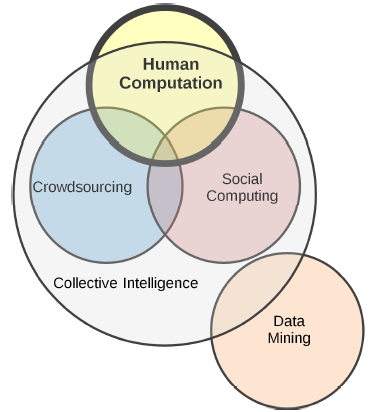
\includegraphics[width=0.6\columnwidth]{HC-relation}
    \caption{\acl{HC} relation with CrowdSourcing, Social Computing and Collective
    intelligence.}
    \label{fig:HC-relation}
\end{figure}
\acl{HC} is related with other terms, such as \emph{CrowdSourcing},
\emph{Social Computing} and \emph{Collective Intelligence} as depicted in
\autoref{fig:HC-relation}. Here we give some definitions to better understand the
similarities and the differences:
\begin{description}
    \item[CrowdSourcing] is "\emph{the act of taking a job traditionally
    performed by a designated agent (usually an employee) and outsourcing it to an
    undefined, generally large group of people in the form of an open call}"
    \cite{howe2006rise}. So it does not involve computation directly like \ac{HC}.

    \item[Social Computing] "\emph{describes any type of computing application
    in which software serves as an intermediary or a focus for a social relation}"
    \cite{schuler1994social}. So despite of the name its purpose is not computing.

    \item[Collective intelligence] defined very broadly as "\emph{groups of
    individuals doing things collectively that seem intelligent}".
\end{description}

When dealing with a human crowd the main issue is to engage users to perform tasks.
A user can be motivated to perform a task due to it's nature
(e.g. the task helps finding the cure to some disease) or to the revenue (e.g.
karma\footnote{Reputation points used in \url{www.reddit.com}.}) he/she gets for doing
such task. The most effective way for recruiting and motivating users is to give
them money\footnote{Since the ancient time. TODO ???}. For instance
\citetitle{turk} is an online tool for performing \ac{HIT} in exchange of money
rewards\footnote{The rewards for a single \ac{HIT} can be as low as 0.01\$.}.\\

\begin{figure}[htb]
    \centering
    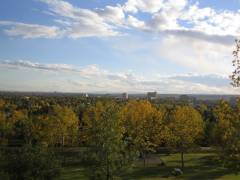
\includegraphics[width=\columnwidth]{HC-distribution}
    \caption{Centralized vs Distributed execution of \acl{HC}.}
    \label{fig:HC-distribution}
\end{figure}
The categorization of \ac{HC} can be further specified by adding another dimension
that involves how the tasks are executed by the users. As you can see in
\autoref{fig:HC-distribution} there are two main types of \ac{HC} execution:
\emph{centralized} and \emph{distributed}.






\subsubsection{Centralized}
In the \emph{centralized} execution we have a central hub (i.e. a website) where
users must go to perform the task. Typically the execution of a task does not
involve the offload of code and data to the user, and there is no need of ad-hoc
softwares to run the task.\\

A good example of a \emph{centralized} \ac{HC} platform is \citetitle{turk}.
\citetitle{turk} is an online platform for executing tasks in exchange of money
rewards. The platform is divided into two sections, one for the \emph{Worker}s and
one for the \emph{Requester}s. The \textbf{Worker}s are users willing to spend
time to execute a \ac{HIT} and receive the reward, the \textbf{Requester}s are
users that publish \ac{HIT} and after getting the results pay the \emph{Worker}s.\\

The lifecycle of a \ac{HIT} is the following:
\begin{enumerate}
    \item A \emph{Requester} creates a \ac{HIT} using one of the predefined project
    instances available.

    \item Once the creation is completed the \ac{HIT} is ready to be executed by
    the \emph{Worker}s.

    \item To execute a \ac{HIT} a \emph{Worker} must visit the \citetitle{turk}
    website and choose from a list of available \ac{HIT}s the one that he/she
    wants to perform (see \autoref{fig:turk}).

    \item Once the whole \ac{HIT} is completed the \emph{Requester} checks the
    result obtained and if he/she is satisfied then proceeds with the payment.
\end{enumerate}
As one can see the whole flow of the \ac{HIT} from the creation to the payment
of the \emph{Worker}s is done within the browser.\\
\begin{figure}[htb]
    \centering
    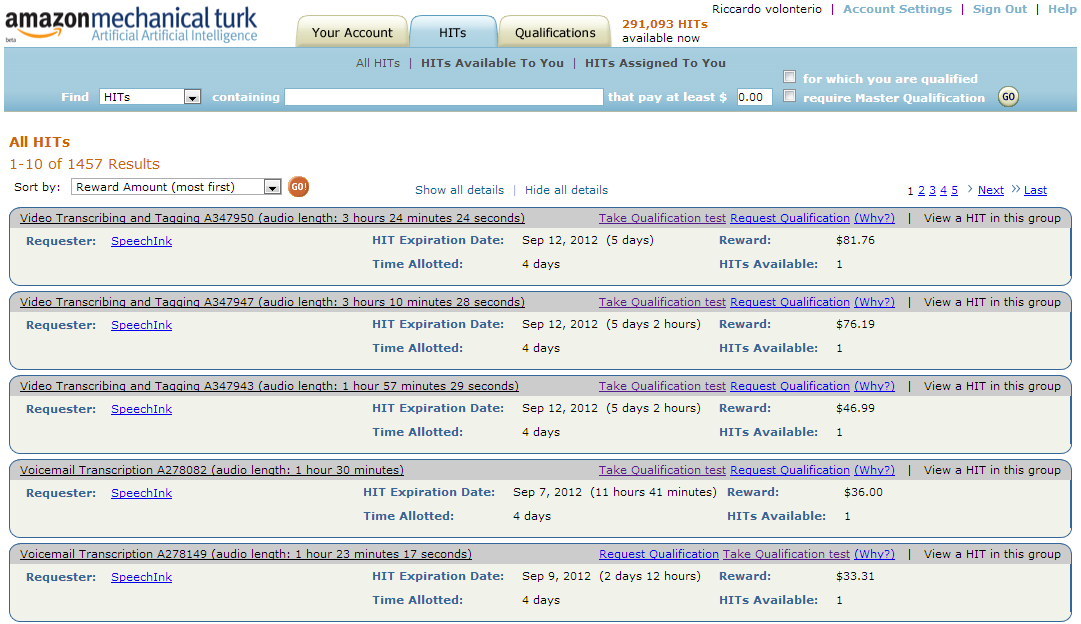
\includegraphics[width=\columnwidth]{turk}
    \caption{\citetitle{turk} web interface for choosing the \acs{HIT}.}
    \label{fig:turk}
\end{figure}


This platform has been \emph{extended} as presented in \cite{little2010turkit}
to create complete \acl{AI} algorithms able to use human computation as functions
during the execution process. The code in \autoref{lst:turkit} is an example of an
algorithm implemented using Turkit. Here \code{mturk.prompt} and \code{mturk.vote}
are \acl{HIT} executed on the \citetitle{turk} platform.
\begin{lstlisting}[language=C++,caption={Example of a Turkit algorithm.},
label={lst:turkit}]
ideas = []
for (var i = 0; i < 5; i++) {
	idea = mturk.prompt("What's fun to see in New York City? Ideas so far: " + ideas.join(", "))
	ideas.push(idea)
}
ideas.sort(function (a, b) {
	v = mturk.vote("Which is better?", [a, b])
	return v == a ? -1 : 1
})
\end{lstlisting}







\subsubsection{Distributed}
In a \emph{distributed} execution environment the central hub acts as a distribution
node in charge of offloading the task upon user request. The user can now run the
task locally without the intervention of the central hub. Eventually, when the task
is done, the user contacts the hub to upload the results.
The process of requesting the task to the hub, executing the task and sending the
results, is all done by the users, typically by a standalone piece of software
installed by the user.

% TODO ??
This solution needs the creation of ad-hoc softwares able to run on every platform
to give users an usable tool for their purpose.\\


\begin{figure}[htb]
    \centering
    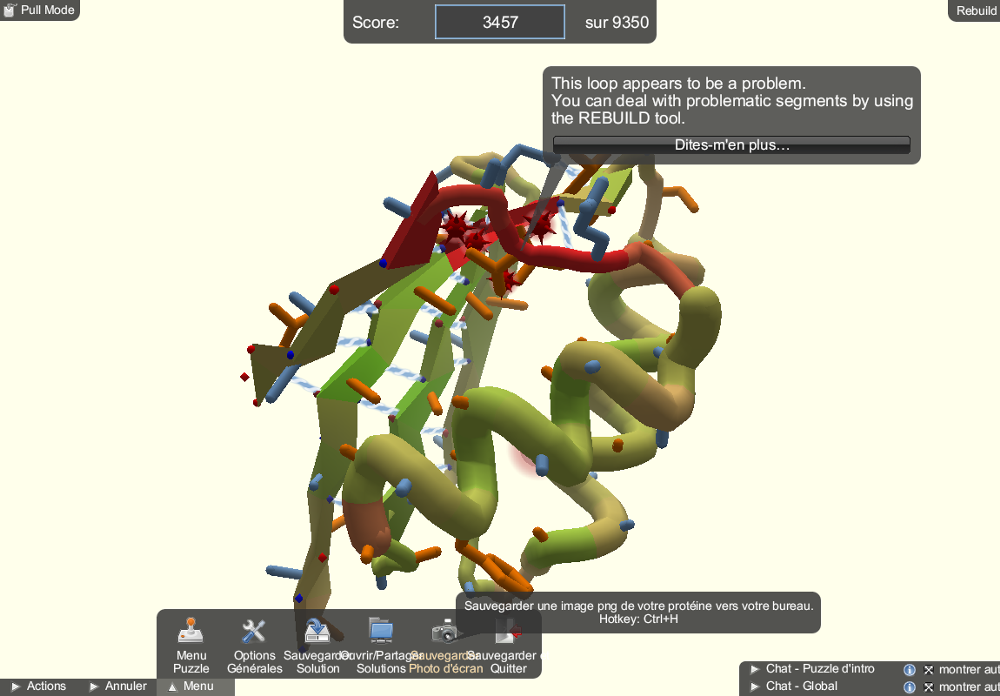
\includegraphics[width=\columnwidth]{foldit}
    \caption{The FoldIt user interface for .}
    \label{fig:foldit}
\end{figure}
An example for this kind of code distribution is the \citetitle{foldit} game.
\citetitle{foldit} is a puzzle game about protein folding, developed
by the University of Washington's Center for Game Science in collaboration with
the UW Department of Biochemistry. The objective of the game is to fold the
structure of selected proteins to the best of the player's ability. The highest
scoring solutions are analyzed by researchers, that can determine whether or not
there is a native structural configuration that can be applied to the relevant
proteins (see \autoref{fig:foldit}).







\subsubsection{\acl{GWAP}}
\acf{GWAP} is "\emph{a human-based computation technique in which a computational
process performs its function by outsourcing certain steps to humans in an
entertaining way}" von Ahn.
\ac{GWAP} come from a simple observation of data on how many hours are spent
playing games. \cite{von2008designing} reported that, accordingly to the
Entertainment Software Association\footnote{Game data from
\url{www.theesa.com/facts/gamer_data.php}}, more than 200 million hours are spent
each day playing computer and video games in the U.S.. Indeed, by age 21, the
average American has spent more than 10,000 hours playing such games equivalent
to five years of working a full-time job 40 hours per week.\\

The simple idea behind \ac{GWAP} is \emph{why not make playing games useful}?
If a task can be transformed into a game the user can be motivated to play the
game so there is no need of other types of reward (i.e. money) for doing such
task. The entertainment of playing the game itself can be used as a reward for
the user.\\

The ESP game, is a \ac{GWAP} developed by Luis von Ahn to perform image tagging.
The users' task is to agree on a word that would be an appropriate label for the
recognition of the image as described in \cite{von2004labeling}. Another \ac{GWAP}
by von Ahn is Peekaboom, where users help computers locating objects in images.

\subsection{Automatic computation}
\label{sec:bg:crowd:auto}

Unlike human computation, \emph{automatic computation} aims at executing a task, or
part of it, in an automatic fashion, without user's interaction. This kind of
\emph{distributed computation} leverages on the existence of a \emph{grid} of
connected nodes able to perform data intensive calculation.


Distributed computing deals with the execution of code on multiple computers
connected to a network. As stated in \cite{andrewsfoundations}: "\emph{Distributed
computing is a field of computer science that studies distributed systems. A
distributed system consists of multiple autonomous computers that communicate
through a computer network. The computers interact with each other in order to
achieve a common goal. A computer program that runs in a distributed system is
called a distributed program, and distributed programming is the process of
writing such programs.}"
\begin{figure}[htb]
    \centering
    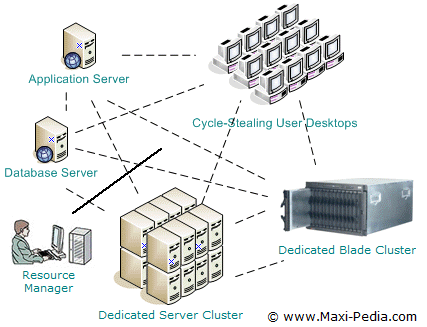
\includegraphics[width=\columnwidth]{DistributedComputing}
    \caption{General structure of a distributed computing system.}
    \label{fig:distributed-computing}
\end{figure}

% TODO ???
The platforms that implement these solution use different frameworks for splitting
algorithms into atomic operation executable by the nodes. One of these frameworks
is MapReduce\footcite{dean2008mapreduce} that, using the core concept of
\emph{Divide et impera}, can produce highly parallelizable algorithms.\\

The name "\emph{distributed computing}" refers to a wide range of different
applications (i.e. grid computing, cloud computing,
\nameref{sec:bg:crowd:auto:parasitic}, jungle computing\footnote{Winner of the
coolest name 2012}), that implement the same paradigm with different purposes.
Using the dimensions presented in \autoref{tab:matrix} we can divide the
core concept of \emph{distributed computing} into two subcategories: \emph{voluntary
computing} and \emph{parasitic computing}.


\subsubsection{Voluntary computing}
\label{sec:bg:crowd:auto:voluntary}
\emph{Voluntary computing} refers to all those \emph{distributed computation}
systems where the computation is performed on behalf of the users will. In such
systems users go to the website of the "project" they intend to support and, usually
by installing an ad-hoc client, give the resources (i.e. CPU idle time, storage,
etc.) of their machines to the chosen "project".\\

The first project implementing such computing paradigm was
\ac{GIMPS}\footnote{\url{http://www.mersenne.org/}}, started in 1995. Then other
platforms (such as \href{http://www.distributed.net/}{distributed.net},
\href{http://setiathome.berkeley.edu/}{SETI@home}, etc. ) have been developed to
support this type of computation.

\begin{figure}[htb]
    \centering
    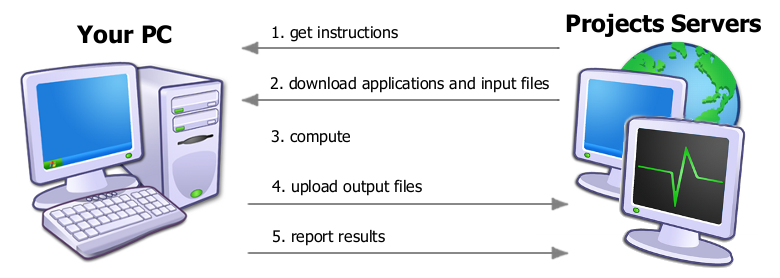
\includegraphics[width=0.8\columnwidth]{boinc}
    \caption{The \acs{BOINC} computational flow.}
    \label{fig:boinc}
\end{figure}
\acf{BOINC}\footnote{\url{http://boinc.berkeley.edu/}} is an open-source software
for Voluntary computing and grid computing. \ac{BOINC} was originally developed
to support the \acf{SETI@home} project, before it became used as a platform for
other distributed computing applications. It consists of two parts: the back-end
server, running on Linux platforms, and the client, cross-platform, for the
end-user computing.\\

The client software allows users to connect to the \ac{BOINC} grid, to perform
computation. The flow of the execution, as depicted in \autoref{fig:boinc} is
the standard \emph{distributed computing}. Here is the list of actions performed
to run the task on the client:
\begin{enumerate}
    \item get instruction from the server on how to get all the resources needed
    to perform the task
    \item download all the resources from the server
    \item execute the downloaded application
    \item send the results obtained to the server
\end{enumerate}

There are over 40, at the time of writing, projects that leverage on
the \ac{BOINC} platform to perform computation on different application areas.
For example the aforementioned \ac{SETI@home} project uses this framework to
search for extraterrestrial intelligence by analyzing the narrow-band radio
signal coming from the Arecibo radio telescope.


\subsubsection{Parasitic computing}
\label{sec:bg:crowd:auto:parasitic}
\input{Capitoli/Background/Parasitic}



\section{Enabling web-based distributed computation}
\label{sec:bg:web}
% Enabling web-based distributed computation

Using the web (i.e. the browser) as a platform for distributing and executing
code implies that we have the available technologies to perform high-level
\emph{computation} and real-time \emph{communication}. These are the requirements
for evaluating the web as a suitable platform for code distribution.\\

\paragraph{Computation} is the key for being able to perform tasks within the
browser. \emph{Computation} can involve any kind of operation on the data, and
the data itself can be of any type. For instance creating an application that
analyzes audio files, or creating a image manipulation program that runs without
external plugins is relatively simple using standard languages (e.g. C, C++,
Java, etc). Until a few years ago it was almost\footnote{Without using strange
interaction between Flash/Silverlight and the browser.} impossible to do it within
a browser.

HTML5 filled the gap that existed between any "standard" language and \js{}
giving the developers access to all the required APIs needed to create fully
functional web-applications. In \ref{sec:bg:web:html5} are presented all the
features, along with some technical details, that have enabled this evolution.\\

There are also initiatives that aim at simplify the deployment of \js{}
application. Since most of the developers have experience on languages other than
\js{} there is the need of porting existing application to the Web.
Projects like \citetitle{emscripten} and \citetitle{gwt}
offer the possibility to write the code directly in C,C++ (\citetitle{emscripten})
or Java (\citetitle{gwt}) and compile it into pure, and optimized, \js{}.

\citetitle{emscripten}, by Mozilla, is a LLVM-to-JavaScript compiler. It takes
LLVM bitcode (which can be generated from C/C++ using Clang, or any other
language that can be converted into LLVM bitcode) and compiles that into \js{}.
Since it is a compiler it offers multiple grades of optimization that reduce the
size of the \js{} file and speedup the computation. The website is full of demos
of the ported application, including games, 2D/3D game engines, various libraries
and also SQLite.

\citetitle{gwt}, by Google, is a development toolkit for building and optimizing
complex browser-based applications. Its goal is to enable productive development
of high-performance web applications without the developer having to be an expert
in browser quirks, XMLHttpRequest, and \js{}.\\



\paragraph{Communication} is being empowered by
introducing \emph{WebSocket}, that enables full-duplex data exchange with the
server, and \ac{CORS} that gives the developers the possibility to make \ac{AJAX}
requests to "foreign" servers (other than \code{localhost}) without the need of
a proxy for forwarding the requests.\\


% TODO non mi convince
The availability of all those technical API gives the possibility to create a
system capable of performing any \emph{Human} or \emph{Automatic} computation
task without the need of external plugins. We used all the features of HTML5
for the computation side of the System. WebSocket are used for real-time task
monitoring and \ac{CORS} are used within the task to request any
external data needed by the application.

\subsection{\acs{HTML}5}
\label{sec:bg:web:html5}
\begin{figure}[htb]
    \centering
    
\includegraphics[width=0.75\columnwidth]{HTML5logos}
    \caption{Official HTML5 logo \& unofficial CSS3 logo.}
    \label{fig:html-logos}
\end{figure}

When speaking of \ac{HTML}5 one, usually, is not only focusing on the markup language
but on a set of web technologies and specifications strictly related to \ac{HTML}5.
This set of technologies includes the \ac{HTML}5 specification itself, the
\ac{CSS}3 recommendations and a whole new set of \js{} APIs. So, first things
first, let us point out the differences:
\begin{description}
	\item[HTML5] refers to a set of semantic tags (like \ctag{footer},
	\ctag{header}, \ctag{article}, \ldots), media tags (like \ctag{video} or
	\ctag{audio}) and the so called Web Form 2.0 alongside with all the "old"
	tags inherited from HTML4. These tags help developers to give semantics to
	the website they make, so the websites can be
	better understood by search engines or HTML parsers (like those used for
	reading the site for blind people).

	\item[CSS3] refers to the presentation layer of the pages. Here are introduced
	specifications including image effects, 3D transformation, new tag selectors, 
	form element validation, etc. The specifications take care also of the new
	devices (like smartphones and tablets) giving the user the \code{media
	queries} to examine the media (screen, print, aural) and provide different
	\ac{CSS} rules.
	
	\item[JS] refers to the \js{} with a new set of API for interacting with the
	new media elements and other tags, as long as API for concurrent computation,
	real-time communication, offline storage, etc.\\
\end{description}

With the advent of \ac{HTML}5, like any new technology, many problems were
resolved and many others have been created. The main issue with using \ac{HTML}5
is the browser compatibility and browser-specific methods.

When browsers start
implementing some \ac{HTML}5 draft feature, since they are not fully standardized
\footnote{In fact HTML5 (at the time of writing) is not yet standardized, its
still a draft. See \url{http://www.w3.org/TR/html5/}}, they prevent the pollution
of the DOM by prefixing the standard method
with a browser specific prefix\footnote{\code{o}: for
Opera, \code{ms}: for Internet Explorer, \code{moz}: for Firefox, and
\code{webkit}: for the WebKit based browser (Chrome and Safari)}(i.e.
\linebreak\code{requestAnimFrame}
can become \code{mozRequestAnimFrame} or \code{webkitRequestAnimFrame}). This prefixing
is particularly common in the \ac{CSS}3 where things becomes awful\footnote{See
CSS animation or gradients for example.}.\\


To avoid browser inconsistency there are plenty of \js{} frameworks for every
purpose. Frameworks like \citetitle{jquery} provide a layer of abstraction between
browser-specific code and the user, giving developers fallbacks for the most
common API and additional features not covered by the standard implementation.
Other frameworks like \citetitle{modernizr} give developers the ability to test
if some \ac{HTML}5 feature is available in the currently used browser and provide
a general fallback system for dynamically load polyfills\footnote{A polyfill is
a \js{} library or third part plugin that emulates one or more HTML5 feature,
providing websites to have a consistent behavior.}.\\


Now are presented the main \ac{HTML}5 features to better understand how they can
be used in this System.





\paragraph{Canvas}
Let's start with the official definition\footnote{Got from the specs:
\url{http://www.w3.org/TR/html5/the-canvas-element.html\#the-canvas-element}}
\begin{quoting}\rm\tt
	The canvas element provides scripts with a resolution-dependent bitmap canvas, which can
	be used for rendering graphs, game graphics, or other visual images on the fly.
\end{quoting}

So the \code{canvas} element is basically a \emph{Canvas}, like the name says, where
one can \emph{paint} anything. On top of this, the \code{canvas} element gives
the developers access to the underlying raw pixel data. Also in the \code{canvas}
element you can \emph{draw} images taken from a \ctag{img} tag or a frame taken
from a \ctag{video} tag.

As one can see now we have all the tools we need to perform image analysis or
video manipulation within the browser. Obviously there are plenty of \js{}
libraries that facilitate the whole process of filtering or, in general, image
manipulation (like \href{http://www.pixastic.com/}{Pixastic} or
\href{http://camanjs.com/}{Camanjs}). Other libraries give you the tools to
create diagrams or charts on the fly (like \href{http://raphaeljs.com/}{Raphaël}
or \href{http://processingjs.org/}{Processingjs}).

The canvas element also provides a 3D context to draw and animate
\footnote{Animations are not natively supported, must be coded separately.}
high definition graphics and models using the WebGL API. This API is maintained
by the \href{http://www.khronos.org/}{Khronos Group} and is based on OpenGL ES
2.0 specifications. On top of these API there are a lot of libraries\footnote{For
a reference see \url{http://en.wikipedia.org/wiki/WebGL\#Developer_libraries}}
made to facilitate development of 3D applications. One of the the most used is
the \href{http://mrdoob.github.com/three.js/}{Three} \js{} library, that can be
used for creating and animating 2D or 3D scenes within the canvas element.








\paragraph{WebSocket}
The WebSocket is an API interface for enabling bi-directional full-duplex client
server communication on top of the \ac{TCP}. It enables real-time
communication between clients and servers, allowing servers to \textbf{push} data
to the clients and obtain \emph{real} real-time content updates.

Like many other \ac{HTML}5 features on top of WebSocket a library that
provides easy access to these functionality as long as fallbacks for old browsers
was built.
\citetitle{socket.io} provides a single entry-point to create a connection to the
server and manage the message exchange, providing fallbacks\footnote{If WebSocket,
are not available the library can use Adobe\reg Flash\reg Socket, AJAX long
polling, AJAX multi-part streaming, Forever Iframe and JSONP Polling} to ensure
cross-browser compatibility.





\paragraph{WebWorkers}\label{html5:workers}
A problem that rises when coding load intensive \js{} application is the single thread nature
of the language. Every script runs in the same thread of the browser window/tab.
This can lead to some unwanted behavior (like browser freezing or a warning
dialog that that alerts the user as in \autoref{fig:browser-slow-dialog}).
\begin{figure}[htb]
    \centering
    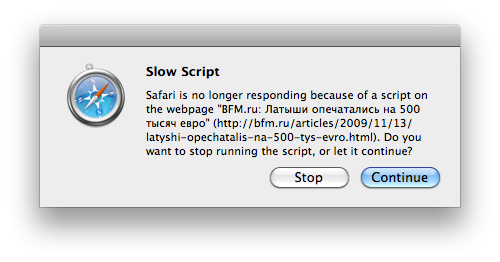
\includegraphics[width=0.75\columnwidth]{browser-slow-dialog}
    \caption{The slow script dialog.}
    \label{fig:browser-slow-dialog}
\end{figure}
To solve this problem \cite{jenkin2008parasitic} proposed a timed-based
programming structure that ensures that the code runs without any browser warning
or freezing and also offers the developer to tweak the performance of the script
by dynamically adjusting the interval between the step execution. This method
leverage on the \code{setTimeout} function of \js{} in order to split code into
timestep-driven code chunks to execute. Here is an example of loop translated
into a timer-based loop:
\begin{multicols}{2}
	\begin{algorithm}[H]
		\While{condition}{
			...do something...
		}
	\end{algorithm}

	\vfill
	\columnbreak

	\begin{algorithm}[H]
		\SetKwBlock{procedure}{procedure}{}
		\SetKwFunction{setTimeout}{setTimeout}

		\procedure(STEP){
			...do something...\\
			\If{condition}{
				\setTimeout{STEP, delay}
			}
		}
	\end{algorithm}
\end{multicols}
Obviously this is not the solution to the problem, it is a hack that tricks the
browser.\\


WebWorkers offer a simpler solution. They provide a simple, yet powerful, way of
creating \emph{threads} in \js{}. The official definition says:
\begin{quoting}\rm\tt
	The WebWorkers specification defines an API for running scripts in the
	background independently of any user interface scripts.	This allows for
	long-running scripts that are not interrupted by scripts that respond to
	clicks or other user interactions, and allows long tasks to be executed
	without yielding to keep the page responsive.
\end{quoting}

The core concept behind WebWorkers is the \code{Worker}. A \code{Worker} is a
piece of \js{} code that runs in parallel to the main thread and is able to send
and receive messages (just like normal threads).



\paragraph{Storage}
When web developers think of storing anything about the user, they immediately
think of uploading to the server. \ac{HTML}5 changes that, as there are now
several technologies allowing the \ac{RIA} to save data on the client device.

\ac{HTML}5 supports a number of storage techniques able to store data within the
browser to be accessed later. Here is a simple list with the principal features:
\begin{description}
	\item[Web storage] is a convenient form for offline storage. It uses a simple
	key-value mapping for storing data persistently on the browser.

	\item[Web SQL database] is an offline SQL database, usually implemented using
	SQLite, a general-purpose open-source SQL engine.

	\item[IndexedDB] is a nice compromise between Web Storage and Web SQL Database.
	Like the former, it is relatively simple and like the latter, it's capable
	of being very fast. It uses the same mapping as \emph{Web storage} and indexes
	certain fields inside the stored data.

	\item[Filesystem API], as the name says, offers the ability to manipulate the
	file system of the host.
\end{description}


\paragraph{Offline storage}
In this category falls the \code{application cache}. The \code{application cache} is
controlled by a plain text file called a \code{manifest}, which contains a list
of resources to be stored for use when there is no network connectivity. The list
can also define the conditions for caching, such as which pages should never be
cached and even what to show the user when he follows a link to an uncached page.

If the user goes offline but has visited the site while online, the cached
resources will be loaded so the user can still view the site in a limited form.
Here is a simple cache file:
\begin{lstlisting}[language=make]
CACHE MANIFEST
      
# This is a comment

CACHE:
/css/screen.css
/css/offline.css
/js/screen.js
/img/logo.png

http://example.com/css/styles.css

FALLBACK:
/ /offline.html

NETWORK:
*
\end{lstlisting}


\subsection{WebCL}
\label{sec:bg:web:webcl}
With the advent of \ac{GPGPU}, the spreading of multicore CPUs and multiprocessor programming (like OpenMP)
we can see emerging an intersection in parallel computing. This intersection is known as
\textbf{heterogeneus computing}. \ac{OpenCL} is a framework for heterogeneus compute resources and so
\ac{WebCL} is a porting of this technlogy to the web.
% Spiego meglio perchè è nato?

\ac{OpenCL} uses a language based on C99\footnote{A programming language dialect for the past C developed in
1999 (formal name ISO/IEC 9899:1999)} for writing \emph{kernels}, functions that actually execute on OpenCL
devices. 
% come funziona OpenCL

% Problema delle prestazioni - FATTO
The main focus when building high-end web-application like 3D games is responsiveness. Altough \js{}
can be optimized and parallelized (see \vref{sec:bg:web:html5}) it cannot be fast as an application
software, because \js{} must be interpreted by the browser and then executed as machine code. \ac{WebCL}
provide an easy framework for building and running machine code in parallel directly from the browser.

% Implementazioni
%% common API 
% prestazioni, esempi
% integrazione con webGL

%************************************************
%\chapter{A model for distributed web-based human- and machine-driven computation}
\chapter{The Model}
\label{cap:model}
%************************************************


% il mio sistema ha una logica di associazione del task
% quale task a chi e con quale codice


% Cubrick METADATA MODEL!!!!!!!!
% definisco l'architettura, chi sono gli attori
% definisco il modello degli attori (task, utente, uTask, client) e come sono relazionati
% ES
% relazione n->n task client
% Il task può essere svolto da codici diversi in funzione del client


% in questo capitolo definiamo il modello del nostro sisstema diviso in
% modello architetturale, modello dei dati e modello di esecuzione
% infine presentiamo la logica di pluggabilità delle strategie (quelle
% di default e quelle custom)











% TODO: cambiare il nome: no system model!
\newcommand{\model}{\emph{architectural model}}
In this chapter, we define the \model for our system and the reference
infrastructure supporting this model.
The \model is the data model on which the single components of the system are build upon.
It describes the components that interact each other during the task lifecycle and
embodies also the requirements and the features of the system as expressed in
the \hyperref[intro]{introduction}.\\



Concerning the data model we have subdivided it in 3 parts, this subdivion is made to
better distinguish each of the 3 main steps used in every distribution system in order
to create, distribute and process the data. \autoref{fig:model} gives an overview of
the \model that is composed by:
% model subdivision
\begin{description}
	\item[The {\hyperref[sec:model:architecture]{architectural model}}:] describes
	the reference architecture .

	\item[The {\hyperref[sec:model:data]{data model}}:] describes
	all the actors and stakeholders present in our system.
	
	\item[The {\hyperref[sec:model:execution]{execution model}}:] focuses
	on the model of the task and the users with their characteristics and proficiencies.

	\item[{\hyperref[sec:model:strategies]{Pluggable strategies}}:] here
	we focus on the provide some example of usage.
\end{description}



% Sezioni
\section{Architectural model}
\label{sec:model:architecture}
\begin{figure}[htb]
	\centering
	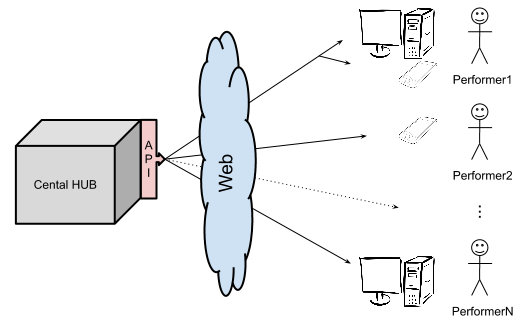
\includegraphics[width=0.75\columnwidth]{Architecture}
	\caption{Reference architecture.}
	\label{fig:architecture}
\end{figure}
% TODO nell'immagine metto anche un dispositivo mobile e un utente con 2 device

During the Design Process we faced the problem of finding a suitable Architectural
Model able to support all the requirements, in terms of flexibility and pluggability,
raised during the Process Design. In our model we use as a reference architecture
the one depicted in \autoref{fig:architecture}. Here we have a central hub
in charge of distributing the Tasks to the nodes\footnote{We refer to nodes
because we want to enclose both humans and devices.} and an abstraction layer.

The \emph{Central Hub} is used to manage all the data exchange between to the
nodes and the hub itself, orchestrating all the communication flow.

The \emph{Abstraction Layer} is used to normalize the differences between the
nodes, creating a coherent representation of nodes.\\




As described in \ref{design:work}, our framework has multiple configuration
points used to customize the Task behavior. As described in \vref{data:task},
for each Task we identified seven configuration points:
\begin{description}
	\item[\utask{} planning strategy:] defines how many \utask{} to create for
	each Task and associate the right portion of Objects to each of them.
	\item[\utask{} implementation strategy:] defines the logic behind the choice
	of a \utask{} implementation sent to a user.
	\item[Performer assignment strategy:] in charge of choosing the users who
	are suitable to execute a certain Task.
	\item[Task Planning strategy:] orchestrates the invocation of the \utask{}
	planning strategy, the \utask{} implementation strategy and the Performer
	assignment strategy.
	\item[Task Control strategy:] defines a controller for the Task, able to
	check the status, and if needed, perform corrective actions.
	\item[Aggregation function:] is in charge of joining the results obtained
	from the \utask{}s execution and create a Task output.
	\item[Emission policy:] is used to rule notifications sent to the Subscribers.
\end{description}
All these configuration points are described in \ref{sec:model:strategies}.

\section{Data model}
\label{sec:model:data}
% Data Model
data model


% task con custom proiperties in modo da configurare i runtime

\section{Execution model}
\label{sec:model:execution}
% Execution model
Execution model

\section{Pluggable strategies assignment}
\label{sec:model:strategies}
%% Pluggable+Strategies

As pointed out during the Process Design and briefly introduced in the 
Architectural Model, our framework must be able to handle custom strategies.
These strategies (see \ref{sec:model:architecture}) are used to grant that
our model is flexible enough to support all the application archetypes
defined in \autoref{tab:matrix}.

This section explains the purposes of each strategy and what are the
main properties for each strategy.


\subsection{\utask{} Planning strategy}
The \utask{} Planning strategy is a pluggable logic devoted to the creation, or
deletion, of \utask{}. Eventually this strategy must, during the creation
time of a \utask{}, bind a corresponding set of Task Objects to the \utask{}.
This binding produce a set of \utask{} with the corresponding Task Objects. A
Task planning strategy is defined by:
\begin{itemize}
    \item A set of \textbf{Constraints} that rules the execution.

    \item A \textbf{Planning policy} that can be defined at:
        \begin{description}
            \item[Design time:] the assignment is made at design time during the
            creation phase. After the planning is done it can be modified only

            \item[Dynamic:] the planning is done at least once, using a provided
            set of input \emph{Object}s. The planning can be further invoked due
            to:
            \begin{itemize}
                \item \emph{Variations} in the state of the Task. i.e. an object
                can be reassigned to another \utask{}.

                \item \emph{Addition} of new \emph{Object}s through the API.
            \end{itemize}
            Note that the addition of new \utask{} can be performed using the
            API but usually do not involve the invocation of a \utask{} planning
            strategy.
        \end{description}
\end{itemize}



\subsection{Performer Assignment strategy}
The Performer assignment strategy is a pluggable logic devoted to the assignment
\emph{Performers} to \utask{}. Once we have a set of \utask{} we can assign to
them the suitable Performers. The Performers are chosen according to some
criteria like their skills or the place they live. A Performer assignment
strategy is composed by:
\begin{itemize}
    \item A \textbf{set of Constraints} defined on top user-specific statistics
	(e.g. do not assign more than 1 \utask{} per hour).

    \item A \textbf{list of routes} that, by matching the description of a
    \emph{Performer}, decide if a \utask{} can be assigned to that \emph{Performer}.

    \item An \textbf{Invitation Strategy}, which defines how performers should be 
    invited to execute the task.

    \item An \textbf{Assignment policy} that can be:
        \begin{description}
            \item[static:] the assignment can be performed both at design time and
            runtime, but it must be explicitly called by a control rule.
            \item[dynamic:] the assignment is performed at least once and can be
            invoked multiple times later according to \emph{Variables} that can
            change over time.
        \end{description}
\end{itemize}



\subsection{\utask{} Implementation strategy}
\utask{} Implementation strategy is a pluggable logic in charge of selecting a
suitable \utask{} implementation for an \emph{Execution}. This strategy is invoked
before the execution of a Task on a device. Based on the Performer preferences
or on the device characteristics a suitable \utask{} implementation is routed to
the user.


\subsection{Task Planning strategy}
The Task Planning strategy embodies the functionalities of a \utask{} Planning
strategy and Performer Assignment strategy, deciding the logic by which the
two strategies should be invoked. This strategy can be used to manage the
re-planning of the \utask{}s or to call the Performer Assignment strategy. The
invocation of this strategy is controlled by the Task Control strategy that can
call this strategy upon changes in the Task status.




\subsection{Task control strategy}
The Task control strategy is a pluggable logic devoted to verifying the status of
a Task, possibly against the assigned constraints. This logic can be executed:
\begin{itemize}
    \item \textbf{Once} when the Task ends. For instance when all the \utask{}s
    are executed to re-plan the execution.

    \item According to a \textbf{temporal schedule} (i.e. every $x$ minutes,
    once a day, at noon, etc.).

    \item Every time a \utask{} is \textbf{executed}.
\end{itemize}
\noindent Among the corrective actions available to the Task controller we have: 
\begin{itemize}
    \item The \textbf{re-planning} of the task, also with the creation of new
    \utask{}.

    \item The \textbf{re-assignment} of \utask{} to \emph{Performer}s.

    \item \textbf{Deletion} of executed \utask{}.

    \item \textbf{Change} the properties of an executed \utask{}. For instance
    we can set the results as invalid if we have spotted a cheater.

    \item \textbf{Re-execution} of the entire Task.

    \item \textbf{Halting} the Task.

    \item etc.
\end{itemize}



\subsection{Aggregation function}
An Aggregation function is a pluggable logic devoted to joining the results
obtained with the \utask{}s execution. These results are merged according to a
Task specific logic in order to produce the Task output result. An aggregation
function can be as simple as a \emph{Sum} or an \emph{Average} but can can also
be more complex. For instance we can gather the results obtained, perform
filtering operation and eventually produce an image.


\subsubsection{Emission policy}
The Emission policy controls how the \emph{Subscribers} are notified about the
status changes in a Task. This logic can be executed:
\begin{itemize}
    \item \textbf{Once} the Task ends.

    \item According to a \textbf{temporal schedule}.

    \item Every time a task is \textbf{executed}.
\end{itemize}

%************************************************
%\chapter{Use cases}
\chapter{Use-cases}
\label{cap:cases}
%************************************************

In the previous chapter we introduced a framework for web-based human and machine
computation, able to handle different types of application archetypes. In this
chapter we present the use-cases use to test this framework under different
scenarios. Since we wanted to test the framework with all the possible application
archetypes we implemented three use-cases: \emph{Automatic}, \emph{Human} and
\emph{Hybrid}:
\begin{description}
    \item[Automatic:] the automatic use-case is used to simulate a
    \emph{Distributed Computing} application. In this scenario we compute the
    SIFT algorithm on an image and return the obtained keypoints to the server.
    \item[Human:] the human use-case is used to test if we can perform \acl{HC}
    with our framework. To test this scenario we implemented a text disambiguation
    application.
    \item[Hybrid:] the hybrid use-case is used to test both the automatic and the
    human scenarios. Here we implemented a \ac{GWAP} on top of a face recognition
    algorithm.
\end{description}
\noindent We focused on the implementation of the \emph{Voluntary} scenario, see
\autoref{tab:matrix}, because the \emph{involuntary} case is almost straightforward
to obtain.
At the end of every use-case will be presented, if possible, a simple
benchmark/metric where the use-case results are compared with the ones obtained
with the available tools. 



\section{Automatic}
\label{sec:cases:automatic}
This use-case is the implementation of the scenario of \emph{voluntary-automatic}
presented in the matrix  in \autoref{tab:matrix}.

For the Automatic use case we choose to implement a widely used feature detection
algorithm, the \ac{SIFT}. To perform this load intensive algorithm we used the
power of the \ac{WebCL} framework to greatly speedup the computation.

% Come funziona
%% Creazione della libreria per comunicare con WebCl
%% Librearia per le operazioni sulle immagini usango WebCL
%% implementazione nella libreria dell'algoritmo
%% Fasi dell'algoritmo


\begin{figure}[htb]
    \centering
    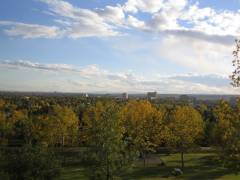
\includegraphics[width=\columnwidth]{Automatic1}
    \caption{The interface of the automatic use-case.}
    \label{fig:Automatic1}
\end{figure}


\begin{figure}[htb]
    \centering
    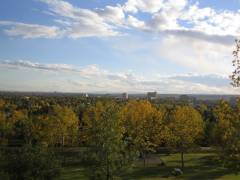
\includegraphics[width=\columnwidth]{Automatic3}
    \caption{Step results of the algorithm.}
    \label{fig:Automatic1}
\end{figure}


\begin{figure}[htb]
    \centering
    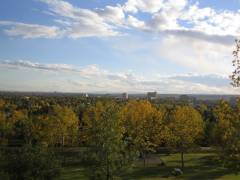
\includegraphics[width=\columnwidth]{Automatic3}
    \caption{Comparison with the reference data.}
    \label{fig:Automatic1}
\end{figure}


% 

%Our scenario is to detect features over 100.000 images using this algorithm


\subsubsection{Benchmark}
%non è possibile una vera comparazione data la velocità

\section{Human}
\label{sec:cases:human}
Dato un testo disambiguarlo usando YAGO (AIDA, https://d5gate.ag5.mpi-sb.mpg.de/webaida/), EntityPedia?, e altri
\citetitle{modernizr}


\section{Hybrid (automatic \& human)}
\label{sec:cases:hybrid}

With the previous sections we presented two applications able to handle the
human and the automatic scenarios. In this section we are presenting a use-case
where both the previous scenarios are blended together. This is used to test
if our framework is flexible enough to seamlessly support mixed application
archetypes. In the matrix at \autoref{tab:matrix} this use-case fits between the
human and the automatic computation.

\begin{figure}[htb]
    \centering
    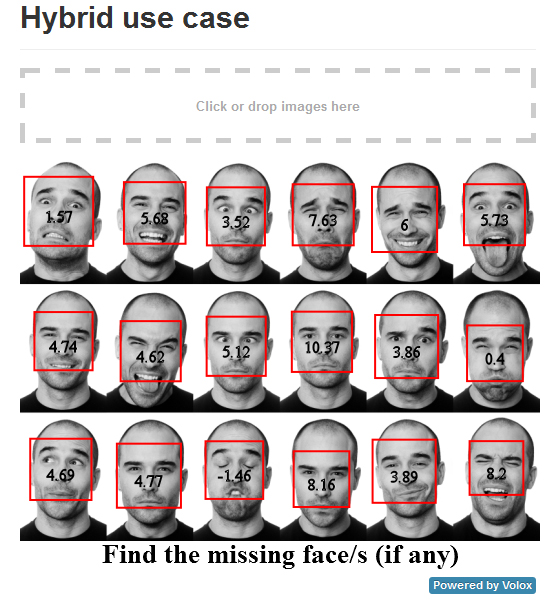
\includegraphics[width=0.75\columnwidth]{Hybrid}
    \caption{Interface of the hybrid use-case.}
    \label{fig:Hybrid1}
\end{figure}

This use-case has the purpose of \emph{detecting faces} in a picture, to accomplish
this Task are used an automatic face recognition algorithm plus a human interaction
that has the double purpose of validating the algorithm result and detect the
missing faces in the image.

This scenario is implemented in 2 steps, in the first step we run the algorithm
for detecting the faces (this is the \emph{automatic} scenario), the second step
is implemented as a \ac{GWAP}.\\

The game, under the name \textbf{ThemAmongUs} has been inspired by the 1988
film "\emph{They Live}" directed by John Carpenter. \emph{ThemAmongUs} is a
single player arcade shooter in which the player assumes a role of an agent that
fights against an alien race disguised as human beings. Equipped with a special
camera able to distinguish between human beings and non humans, the agent is
asked to shoot at the head of the beings that have not been identified by the
camera software. The camera may fail in some occasion, so the agent has to use
his judgment to fire only at the right targets.

\subsection{Introducing Score Degradation}
The new game mechanic that is presented to manage the task is called
Score-Degradation. This technique may be used in scenarios in which there are not
the possibility to compare the results provided by the players with techniques
such as the one provided in output-aggregation or inversion-problems games,
because the game that is being taken into consideration is a not a multiplayer
game but a single player one.

Goal of the technique is to force the user to always provide the right answer
with game mechanics that involve low reaction times , high penalties for mistakes
(such as early game termination) and incentives to achieve the best results
compared to all the other players.

Players are first evaluated based on well known trial examples tasks to understand
their reliability level. Failing the required task in these training examples
usually ends the gaming experience for the player, forcing him to start the game
from the beginning.

Once a sufficient level of trust for the player has been reached, the player is
then provided with a sequence of mixed tasks, some of them with an already well
established knowledge of the expected results, some of them with completely
unknown expected results. While the results of the first kind of tasks will
still be checked against the right results, for the second kind of tasks the
results provided by the players will always be considered good results.

The players will not be able to distinguish which of the instances of the tasks
are being checked against their provided results and which results are simply
considered "true as provided" without any further checks. This behavior is also
enforced by the fact that the player is not able to understand the moment in which
the "trial phase" will end and the fast reaction times force him to not even have
the time to think about providing misleading results, with the risk of having to
start the game from the beginning again.

In this way the player are always forced to try to give the best possible solution
for a specific task. The collected results can be further improved by using
traditional aggregation techniques such as majority voting or similar, depending
on the task that has to be solved.

\subsection{Gameplay}\label{case:hybrid:gameplay}
Goal of the game is to obtain the highest possible score given a limited amount
of time (1 minute). The player is provided with a series of images that present
bounding boxes of the face of human beings automatically identified by the special
camera of the agent. Each provided image will constitute a round of the game. If
in the image some face has not been surrounded by a bounding box, it means that
the portrayed subject is an alien and must be shot at by pressing the left click
button.

The player has a limited amount of time, typically 5 seconds, to shoot at all the
faces that have not been recognized, in order to obtain a certain amount of points.
During a round the player may also find improper bounding boxes, such as knees or
other part of the body that have been recognized as a face.

The player may right click on these boxes to remove them and obtain additional
points. When the player has shoot to all the unboxed faces, he may shoot at a
button on the right lower corner of the screen to play the next round of the game.
The game will end if the player will shoot at a recognized face by mistake.

At the end of each round (after the 5 seconds have passed or when the player has
pressed the end button), the system checks if the player has missed any face. If
it is the case and the image was a trial one or one for which the results were
known, the player will lose the game with a score equal to the number of points
he achieved so far. Otherwise the score for the current round are calculated in
the following way:
\begin{equation}
\begin{split}
    Score &= (RoundNumber*10)*(NumberOfAliensKilled)\\
          &+(100*(FalseBBRemoved))
\end{split}
\end{equation}

At the end of the global gaming time, a player who has not made any mistake will
receive 1000 additional points. The points are used to provide an incentive to
improve and beat other players by improving the score on further matches.


%************************************************
\chapter{Implementation and evaluation}
\label{cap:implementation}
%************************************************

The previous chapters presented the Conceptual Model and the Use-cases of a
framework for web-based human and machine computation. In this chapter are
presented the actual implementation of the framework and the use-cases.
The framework implementation is dived in two parts: the Configurator, managed by
the Crowdsearcher (see \autoref{sec:bg:crowd:cs}), and the Execution Layer
implemented in NodeJS.
The use-cases are built in \js{} and  the Execution Layer and leverages on
the \ac{HTML}5 features described in \autoref{sec:bg:web:html5}.

\section{Architecture}
\label{sec:implementation:arch}
In this section we present the architecture of our framework, whose implementation
is divided in two parts. The reference model in \autoref{fig:architecture} has
been customized to meet our needs in terms of flexibility and pluggability.
As one can see in \autoref{fig:architecture2} the Central Hub has been splitted
into two separated components: the \emph{Configurator} and the \emph{Execution Layer}.
The \emph{Configurator} is in charge of managing the Tasks lifecycle. It is used
to create and configure the Tasks.
The \emph{Execution Layer} is used to configure the actual implementations for
each \utask{}.

\begin{figure}[htb]
    \centering
    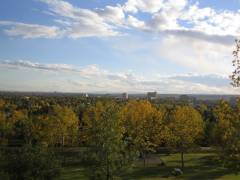
\includegraphics[width=\columnwidth]{Architecture2}
    \caption{Specialized architecture.}
    \label{fig:architecture2}
\end{figure}

\subsection{Configurator}\label{sec:configurator}
The \textbf{Configurator} is in charge of managing the Tasks lifecycle
from the abstract definition to the results aggregation. This component must
implement the metamodel described in \ref{data:model} to describe the Tasks and
must handle correctly the the hooks defined in \ref{sec:model:strategies}. This
component must have a set of API for the Task management.
The main functionality offered by the \emph{Configurator} are:
\begin{itemize}
    \item Allow the \textbf{creation} of a Task, also at abstract level, using
    either the API or the built-in UI.

    \item Allow a \emph{Performer} to \textbf{execute} the Task using a standard
    non configurable UI, provided as-is for each Task type.

    \item Allow to \textbf{request information} about a Task, the information
    that can be requested includes:
    \begin{itemize}
        \item Retrieve the list of \utask{} associated with a given Task

        \item Post the result of the execution of a given \utask{}

        \item Notify about the completion of a Task or \utask{}
    \end{itemize}
\end{itemize}

\noindent For implementing this component we adopted the \emph{CrowdSearcher} framework.
As described in \ref{sec:bg:crowd:cs} this framework natively embodies most of
the functionality described previously. Now we describe the process of creating
and planning a Task. The description is focused on the built-in implementation,
by plugging-in custom sstrategies one can completely change how the framework behaves.

\subsubsection{Task creation}
The task creation if performed by the \emph{Configurator} either by using its
web-interface or via API calls. The creation of a Work/Task can be performed with
three methods: using a JSON file, via API calls or using a step-by-step "manual" procedure.
Using a JSON file, user can supply file containing all the required information like
the data definition and the data instances.
Otherwise the user create the new Task following a step-by-step procedure bundled
with the \emph{Configurator}. As shown in \autoref{fig:task-creation} the manual Task
creation involves the definition of a \textbf{Schema} for the data with all the
related Fields. Once the Schema has been defined the user can supply the data
instances to the Task.

\begin{figure}[htb]
    \centering
    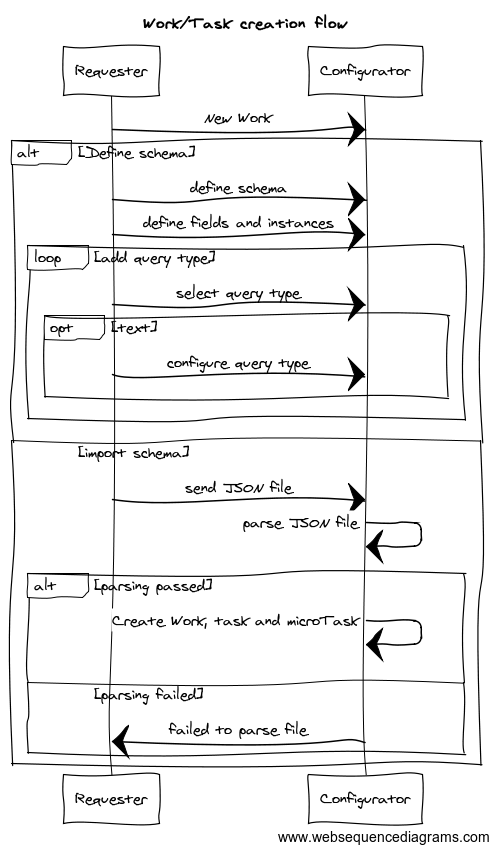
\includegraphics[width=0.65\columnwidth]{task-creation}
    \caption{Work/Task creation flow.}
    \label{fig:task-creation}
\end{figure}



\subsubsection{Task planning}
\begin{figure}[htb]
    \centering
    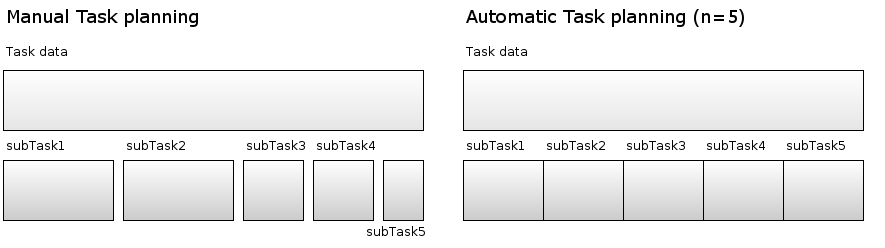
\includegraphics[width=\columnwidth]{planning}
    \caption{Manual Task planning vs Automatic Task planning.}
    \label{fig:auto-manual-planning}
\end{figure}
The planning of a Task involves the creation of \utask{} with the associated data.
The assignment can be performed either automatically or manually.
The automatic plan assignment uses a simple subdivision based on the
number of instances to assign to each \utask{} (see \autoref{auto-manual-planning}).

As depicted in \autoref{fig:task-planning} manual planning involves the
\emph{Requester} interaction in order to create each \textbf{\utask{}}.
After the creation of the \utask{} the user have to select the instances belonging
to this \utask{}. Eventually the user is able to select and, if needed,
configure the type of the \utask{}. The configurable types must be a subset of
the parent Task types.
\begin{figure}[htb]
    \centering
    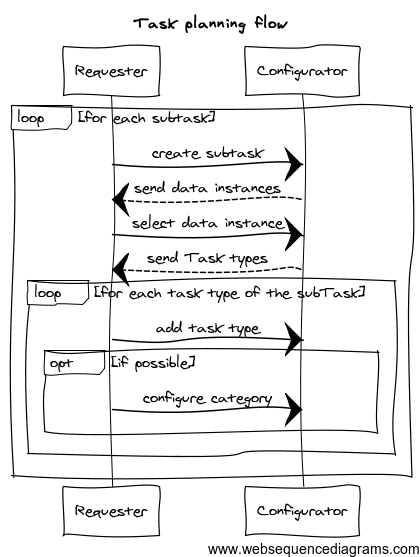
\includegraphics[width=0.65\columnwidth]{task-planning}
    \caption{Task planning flow.}
    \label{fig:task-planning}
\end{figure}










\subsection{Execution layer}\label{sec:exec-layer}
The \emph{Execution Layer} is in charge of managing the \utask{} implementations.
As described in \ref{data:task}, each Task belongs to a macro-type (i.e.
classify, like, comment, etc), and each macro-type  has its own built-in
implementation. The \emph{Execution Layer} give an easy overriding method to
replace the built-in UI with a custom one.
Using the \emph{Execution Layer} a user is able to upload the executable resources
(e.g. HTML, \js{}) that will be used as the new interface.
This custom implementations can be defined hierarchically for Work, Task
and \utask{}. So we can supply custom code for the whole Task or
for each \utask{}. Using this system we have the ability to tweak single
Tasks without harming the others. The layer provides a fallback
system for finding the most suitable code for each \utask{}.

The \textbf{Execution layer} offer the following functionalities:
\begin{itemize}
    \item Allow a \emph{Requester} to configure the implementations associated to
    a Task and/or a \utask{}. The implementations are configured specifying the
    target platform (mobile, desktop, tablet, ...) and the executable resources
    used by the implementation (i.e. HTML, CSS and JS files). Which implementation
    to use is configured later in the \emph{Planning} step.

    \item Create a layer of abstraction between the implementation and the
    Configurator, creating a sandboxed environment where the implementation can
    run and communicate with the Configurator.

    \item Allow the \emph{Performer} to execute a specific \utask{} implementation.
\end{itemize}

\noindent The \emph{Execution Layer} has been developed using \citetitle{node}.
\citetitle{node} is a platform built on Chrome's \js{} runtime for easily building fast,
scalable network applications. \citetitle{node} uses an event-driven, non-blocking I/O model
that makes it lightweight and efficient, perfect for data-intensive real-time
applications that run across distributed devices. Due to the great hype
around \citetitle{node} and the ease of developing new libraries, there are
thousands of these being developed and made available via the built-in
package manager \code{npm}.\\

The implementation of the \emph{Execution Layer} is subdivided into two parts:
the \emph{Server Backend} and the \emph{\utask{}s Wrapper}.

\paragraph{Server Backend} is a node REST web-server implemented using
\citetitle{express}. This server provides an web interface for managing the
implementations of Tasks and \utask{}s. This interface allows a user to upload
custom code (e.g. HTML, JS, CSS) for the selected Task (or \utask{}).
The Server interacts with the \emph{Configurator} to gather information on
a Task composition and type.

\paragraph{\utask{}s Wrapper} exposes a wrapper class that can be used by the
\utask{}s implementations to communicate with the \emph{Server Backend}. The
envelops the \utask{} and supply useful methods to retrieve Task configurations,
gather the associated data and post the results \emph{Configurator}.\\





\subsection{Task storage \& task runtime storage}
These are the storage areas where we put all the data associated with the Tasks
and the \utask{}s implementations. We used two separated storage area to physically
separate the runtime data from the abstract configuration of the Task.

The \emph{Task Storage} is handled by the \emph{Configurator}, meanwhile the
\emph{Task Runtime Storage} is managed by the \emph{Execution Layer}.\\



\subsection{Performer \& Performer Client}
The \emph{Performer client} represents the platforms (like desktop or mobile) on
which a \emph{Performer} executes a Task implementation. The \emph{Performer
client} make use of the \emph{Execution layer} API to retrieve the correct
implementation, communicate the status during the execution of a \utask{} and
post the result of the execution. The \emph{Performer} is the actual user that
is using the \emph{client}.






















\section{Use cases}
\label{sec:implementation:use-cases}

The previous section presented the implementation of the framework described in
this thesis. Now we describe the implementation of the three use-cases described
in \ref{cap:cases}: Automatic, Human and Hybrid.

\subsection{Automatic}
With this scenario we want to test if the browser is able to perform CPU
intensive application. As described in \ref{sec:cases:automatic} in this
scenario we are implementing the \acf{SIFT} algorithm. This algorithm
was chosen due to its high computational requirements.

We made some preliminary tests to check if we can implement this algorithm using
pure \js{} code but we stumbled across the problems described in
\nameref{html5:workers}. Due to this limitation we opted to implement the
code using \ac{WebCL} (see \ref{sec:bg:web:webcl}). With this framework we can
leverage on the \ac{GPGPU} power to perform the computations and unburden the
\js{} engine.\\ 

In order to build a working example of the algorithm we started with the creation
of an \emph{Abstraction Layer} over the \ac{WebCL} raw implementation. Then we created
a small \emph{MultiMedia Library} able to interact with the \emph{Abstraction
Layer} for performing the CPU intensive operations. Eventually we implemented the
\ac{SIFT} algorithm within the \emph{MultiMedia Library}.

\paragraph{The abstraction layer} allow an easy communication with the \ac{WebCL}
framework. As described in \ref{sec:bg:web:webcl}, for running a OpenCL/WebCL
program a few step must be performed. Here is the list:
\begin{enumerate}
    \item Query host for \ac{OpenCL} devices.
    \item Create a context to associate \ac{OpenCL} devices.
    \item Create programs for execution on one or more associated devices.
    \item From the programs, select kernels to execute.
    \item Create memory objects accessible from the host and/or the device.
    \item Copy memory data to the device as needed.
    \item Provide kernels to the command queue for execution.
    \item Copy results from the device to the host.
\end{enumerate}
\noindent Our \emph{Abstraction Layer} allow to define all the I/O parameters
first and then run the selected \code{kernel} function on top of these. This abstraction
allowed us to easily interact with \ac{WebCL} without performing all the previous
steps each time we need to execute a \code{kernel} function.


\paragraph{The MultiMedia library} is a set of image operations implemented using
both \js{} and the OpenCL kernel language. With this library we provided a minimal
set of common operations (e.g. convolve, blur, resize, etc.) useful for the
implementation of the \ac{SIFT} algorithm.\\

\paragraph{The algorithm} has been implemented using the methods of the
\emph{MultiMedia library}. The algorithm has been implemented step-by-step
as described in \ref{case:auto:sift}. For each step the intermediate result
is stored and the step itself is timed to find bottlenecks. In
\autoref{fig:Automatic2} and \autoref{fig:Automatic3} are presented the
intermediate results obtained during the process and the final result.
\begin{figure}[htb]
    \centering
    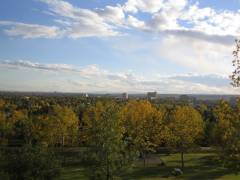
\includegraphics[width=\columnwidth]{Automatic2}
    \caption{Intermediate results of the algorithm.}
    \label{fig:Automatic2}
\end{figure}

\begin{figure}[htb]
    \centering
    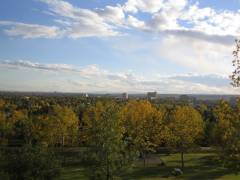
\includegraphics[width=\columnwidth]{Automatic3}
    \caption{\acs{SIFT} result comparison with the reference data.}
    \label{fig:Automatic3}
\end{figure}





\subsubsection{Benchmark/Metric}
Since the purpose of this use-case is the feasibility of high load computation
on the user browser, the implementation of the algorithm has not been optimized.
Then the performance of this implementation are not comparable to the existing
C/C+ implementation+, but we can leverage on the parallelism of the whole
framework to obtain an higher throughput. In our test cases we obtained the
results presented in \autoref{tab:auto-data}.
\begin{table}[htb]
    \caption{\acs{SIFT} algorithm performances.}
    \label{tab:auto-data}
    \centering
    \begin{tabular}{c|c|c|c}
        \textbf{Image size} & \textbf{ScaleSpace + Dog} & \textbf{Keypoints
        detection} & \textbf{Total time}\\
        \hline
        1024x683 & \textasciitilde{}4300 ms & \textasciitilde{}1100 ms & \textasciitilde{}5400 ms\\
        \hline
        800x534 & \textasciitilde{}2600 ms & \textasciitilde{}700 ms & \textasciitilde{}3400 ms\\
        \hline
        600x401 & \textasciitilde{}1500 ms & \textasciitilde{}360 ms & \textasciitilde{}1900 ms\\
        \hline
        400x360 & \textasciitilde{}1130 ms & \textasciitilde{}310 ms & \textasciitilde{}1500 ms\\
        \hline
    \end{tabular}
\end{table}

















\subsection{Human}
The Human





















\subsection{Hybrid}
In this scenario we have the human and the automatic computation blended together.
As explained in \ref{sec:cases:hybrid}, this use-case is implemented in two
parts: the face detection and the \ac{GWAP} logic.\\

The face detection logic is implemented using an external library by
\href{http://liuliu.me/}{Liu Liu}. This library allow to detect face in an image
using the \js{} features presented in (like \code{Canvas} and \code{WebWorkers}).
The technique used to implement the algorithm will not be covered here but you
can find a detailed explanation here:
\url{http://liuliu.me/eyes/javascript-face-detection-explained/}.
The library\footnote{Source code: \url{https://github.com/liuliu/ccv/tree/unstable/js}}
can be used with or without WebWorkers to further increase the processing
speed\footnote{Demo available here: \url{http://liuliu.me/ccv/js/nss/}}.\\

The \ac{GWAP} follows the game logic presented in \ref{case:hybrid:gameplay} an
it has been implemented using the \ac{HTML}5 features.
\appendix
%************************************************
\chapter{Conclusion and future works}
\label{cap:conclusion}
%************************************************

In this thesis we proposed a novel approach for web-based human and machine
computation. By leveraging on the features offered by the modern web browsers,
we provide a framework for designing and implementing general purpose Tasks.
This system allows the user to configure the Task at abstract level and add
all the required custom implementations later, even during the execution.
On top of that our framework offer the possibility to plugin external
logic to tweak the Task execution flow. With this pluggable behavior our framework
is able to support any application archetype (human, automatic and hybrid).

Eventually during this thesis we described three use-cases. This scenarios were
used to evaluate our framework and to test whether the web can be used as a
platform for general Task execution.

\section{Future work}
The described work reveals the hidden potential of the modern web. Our framework
can be extended to meet the scenario proposed by \cite{karame2011pay}. Here we
can use the features of our framework to create an online marketplace for exchanging
computation to contents. Here is a list of other possible enhancements to our work:
\begin{itemize}
    \item Better support for image processing with optimized libraries.
    \item Enhanced Task creation with the implementation of wizards that guide
    the user though the Task creation.
    \item Enriching of the framework with the addition of supported application
    archetype.
\end{itemize}
% *****************************************************************
% Materiale finale
%******************************************************************
%\backmatter
\section*{Acronyms}
\begin{acronym}[WYSIWYG]

    \acro{WebCL}{Web Computing Language}

    {\small The WebCL working group is working to define a JavaScript binding to the Khronos \ac{OpenCL}
    standard for heterogeneous parallel computing. WebCL will enable web applications to harness GPU and
    multi-core CPU parallel processing from within a Web browser, enabling significant acceleration of
    applications such as image and video processing and advanced physics for \ac{WebGL} games.\par}

    \acro{SIFT}{Scale-Invariant Feature Transform}

    {\small SIFT is an algorithm in computer vision to detect and describe local features in images.\par}


    \acro{OpenCL}{Open Computing Language}

    {\small OpenCL is a framework for writing programs that execute across heterogeneous platforms consisting
    of CPU, GPU, and other processors. OpenCL includes a language (based on C99) for writing \emph{kernels}
    (functions that execute on OpenCL devices), plus APIs that are used to define and then control the platforms.
    OpenCL provides parallel computing using task-based and data-based parallelism.\par}

    \acro{WebGL}{Web Graphics Library}

    {\small WebGL is a cross-platform, royalty-free API used to create 3D graphics in a Web browser. Based on
    OpenGL ES 2.0, WebGL uses the OpenGL shading language, GLSL, and offers the familiarity of the standard OpenGL API.
    Because it runs in the HTML5 Canvas element, WebGL has full integration with all DOM interfaces.\par}

    \acro{CORS}{Cross-origin Resource Sharing}

    {\small Cross-origin resource sharing (CORS) is a web browser technology specification which defines ways
    for a web server to allow its resources to be accessed by a web page from a different domain. Such access
    would otherwise be forbidden by the same origin policy. CORS defines a way in which the browser and the
    server can interact to determine whether or not to allow the cross-origin request. It is a compromise
    that allows greater flexibility, but is more secure than simply allowing all such requests.\par}

    \acro{RIA}{Rich Internet Application}

    {\small Rich Internet Applications (RIA) are web-base application that have many of the characteristics of
    desktop application software. \par}

    \acro{HIT}{Human Intelligent Task}
    \acro{HC}{Human Computation}
    \acro{AI}{Artificial Intelligence}
    \acro{GIMPS}{Great Internet Mersenne Prime Search}

    \acro{TCP}{Transmission Control Protocol}
    
    \acro{JSON}{JavaScript Object Notation}

    \acro{AJAX}{Asynchronous JavaScript and XML}

    \acro{HTML}{HyperText Markup Language}
    \acro{CSS}{Cascading Style Sheets}

    \acro{BOINC}{Berkeley Open Infrastructure for Network Computing}

    \acro{GWAP}{Game With A Purpose}

    \acro{GPGPU}{General-purpose computing on graphics processing units}
    \acro{SPMD}{Single process/program multiple data}
    \acro{SIMD}{Single instruction multiple data}

    \acro{SETI@home}{Search for Extra-Terrestrial Intelligence \emph{at} home}

    {\small SETI@home is an Internet-based public volunteer computing project employing the BOINC software
    platform, hosted by the Space Sciences Laboratory, at the University of California, Berkeley, in the United States.
    Its purpose is to analyze radio signals, searching for signs of extra terrestrial intelligence, and is one of
    many activities undertaken as part of SETI.\par}

    \acro{DoG}{Difference of Gaussian}
\end{acronym}
% !TEX encoding = UTF-8 Unicode
% !TEX TS-program = pdflatex
% !TEX root = ../Tesi.tex
% !TEX spellcheck = it-IT

%*******************************************************
% Bibliografia
%*******************************************************
\cleardoublepage
\nocite{*}

\defbibheading{base}{\subsection*{\bf Essential bibliography}}
\defbibheading{online}{\subsection*{\bf Online resources}}

\printbibliography[heading=base,nottype=online]
\printbibliography[heading=online,type=online]

%% !TEX encoding = UTF-8 Unicode
% !TEX TS-program = pdflatex
% !TEX root = ../Tesi.tex
% !TEX spellcheck = it-IT

%*******************************************************
% Dichiarazione
%*******************************************************
\cleardoublepage
\phantomsection
\pdfbookmark{Dichiarazione}{Dichiarazione}
\chapter*{Dichiarazione}
\thispagestyle{empty}
Dichiaro che questa ricerca è opera mia, ad eccezione delle parti esplicitamente menzionate nel testo, e che questo lavoro non è stato proposto per alcuna qualifica accademica o professionale, ad eccezione di quanto esplicitamente dichiarato.

Dichiaro inoltre che il materiale contenuto in questo lavoro può essere pubblicato, tutto o in parte, dal mio Relatore di tesi di laurea in Matematica, Prof.~Ermanno Lanconelli, dell'Università di Bologna.

\bigskip
 
\noindent\textit{\myLocation, \myTime}

\smallskip

\begin{flushright}
    \begin{tabular}{m{5cm}}
        \\ \hline
        \centering\myName \\
    \end{tabular}
\end{flushright}

\end{document}
